\documentclass{article}
\usepackage{tikz}
\usepackage{array}
\usepackage{calc}
\usepackage{setspace}
\usepackage{amsmath}
\usepackage{xspace}
\usepackage{color}
\usepackage{pgfplots}
\usetikzlibrary{shapes.geometric, arrows}

\tikzstyle{startstop} = [rectangle, rounded corners, minimum width=3cm, minimum height=1cm,text centered, draw=black, fill=red!30]
\tikzstyle{io} = [trapezium, trapezium left angle=70, trapezium right angle=110, minimum width=3cm, minimum height=1cm, text centered, draw=black, fill=blue!30, text width = 2cm]
\tikzstyle{process} = [rectangle, minimum width=3cm, minimum height=1cm, text centered, draw=black, fill=orange!30, text width = 2cm]
\tikzstyle{decision} = [diamond, minimum width=3cm, minimum height=1cm, text centered, draw=black, fill=green!30, text width = 2cm]
\tikzstyle{arrow} = [thick,->,>=stealth]
\pgfplotsset{width=10cm,compat=1.9}

\newcommand\mTW{1.5cm}
\newcommand{\TODO}[1] {{\color{red}\textbf{TODO: #1}}}

\begin{document}
\title{XSgen}
\date{January, 25, 2017}
\author{Flanagan, Robert \and Scopatz, Anthony}
\maketitle
\onehalfspacing

\section{Introduction}
Reactor simulation is an essential part of nuclear engineering. There are three main divisions of reactor modeling strageties; low, medium, and high fidelity. Each of these models provides different benefits to a simulation but comes with costs to either accuracy or computational time.  

Low fidelity models are those models that include no physics at run time. These types of models work for systems that have fixed behaviors. For example, a reactor during steady state operation. One type of low fidelity model is a recipe reactor. These models use fixed input and output recipes. This means that they can simulate a reactor with a single computational operation. Some low fidelity models include interpolation techniques to build libraries on the fly. For example, interpolating between recipes for 3\% enriched fuel, and 4\% enriched fuel might be used to get a 3.5\% enriched fuel recipe. However, interpolating like this fails to directly capture any of the physical changes that might happen to the core by switching from either 3\% or 4\% enriched fuel to a 3.5\% fuel.

High fidelity models are performed using neutronics calculations and bateman equation solvers. These models tend to require details on the entire reactor design to set up. Additionally, due to the necessity to simulate a large number of neutrons to produce higher accuracy, these models require a heavy amount of computation to complete. An example of a high fidelity reactor model is the MCNP\cite{mcnp5monte} burn card which couples MCNP's Monte Carlo simulation with a depletion calculator.   

Medium fidelity models are those that include physics calculations (not including full neutronics calculations) during their operation. These models typically work off datasets that are built ahead of time using higher fidelity models. The physics they incorperate uses the information in these datasets, or outside sources (cross section data, reactor design data, etc.) to modify the data in the datasets and increase the fidelity of the results. Examples of these medium fidelity models are Class\cite{class}, and Bright-lite\cite{brightlite}\cite{flanagan}. 

These medium fidelity models can incorperate a number of different techniques to perform their tasks. Bright-lite, for example, uses a fluence based neutron balance approach to determine the behavior of the reactor. It also includes some optional physics behaviors such as disadvantage factors, batch physics, and fuel blending. Class, on the other hand, uses a set of reactor input and output recipes and machine learning to determing reactor behavior. To understand how these different modeling choices impact a fuel cycle, or the isotopic behavior of a reactor type, it is important for the models to all start from the same base information. 

At present, medium fidelity models use different methods for generating their datasets. This means that any comparison between their methods would be invalid because they all start from different places. Any difference in their final results could be derived from either their data generation step or their methodology. Therefore, only an analysis that uses the same baseline data generation across multiple software is useful for determining any differences in their behavior. 

This work discusses a methodology, know as XSgen, that aims to provide a basis for generation of datasets that medium fidelity models could use to create canonical sets of data. 

XSgen links several peices of software together to automate the generation of medium fidelity model datasets. The first piece of software is a high fidelity neutronics code. XSgen uses OpenMC as the software to perform this step. Flux is extracted from OpenMC\cite{class}. This is used by a cross section calculation software to generate one-group or multi-group cross-sections. This operation is performed by Python for Nuclear Engineers (PyNE)\cite{pyne}. Finally, using either the one-group or multi-group cross-sections, a depletion solver is employed. Currently this role is completed by Origen2.2\cite{origen2}, and therefore one-group cross-sections are required.  

This set of software is capable of providing the inputs that medium fidelity models could use; time dependent one group cross-sections, time dependent multi-group cross-sections, transmutation matricies, burnup rates, etc. XSgen stores the outputs of each of these software into a single large database, from there medium fidelity models can extract the information they need to derive a new dataset for use. This process is currently automated for only Bright-lite.

XSgen can also be used to set up more accurate comparisons between low fidelity model types, specifically recipe reactors, and medium fidelity reactor model types. This is made possible because XSgen can simulate a fuel bundle well past its effective lifetime in the core. The data generated by an XSgen run of this type contains enough information to build out an estimate of core isotopics at discharge using some reactor batch physics discussed later.

\section{XSgen Workflow}
The XSgen workflow is composed of three main parts as mentioned above; OpenMC, PyNE, Origen2.2. The first step is the simulation of the reactor core using a Monte Carlo neutron transport simulation. The main result of this is the flux spectrum. The spectrum is then collapsed with a a cross section database and converted into a suite of one group cross sections for a reactor at a given time $t$ (days) after the reactor has started up. These one group cross sections are then used inside of
a Bateman equation solve to calculate the burnup, neutron production, neutron destruction,
and transmutation matrices. The value of $t$ is set by the user when XSgen is executed.
The composition of the material at the end of the time step is then submitted back to
the Monte Carlo simulator as input. This process is repeated until the maximum time
step specified is reached. This flow is displayed in Figure \ref{fig:flow}.

\begin{figure}\center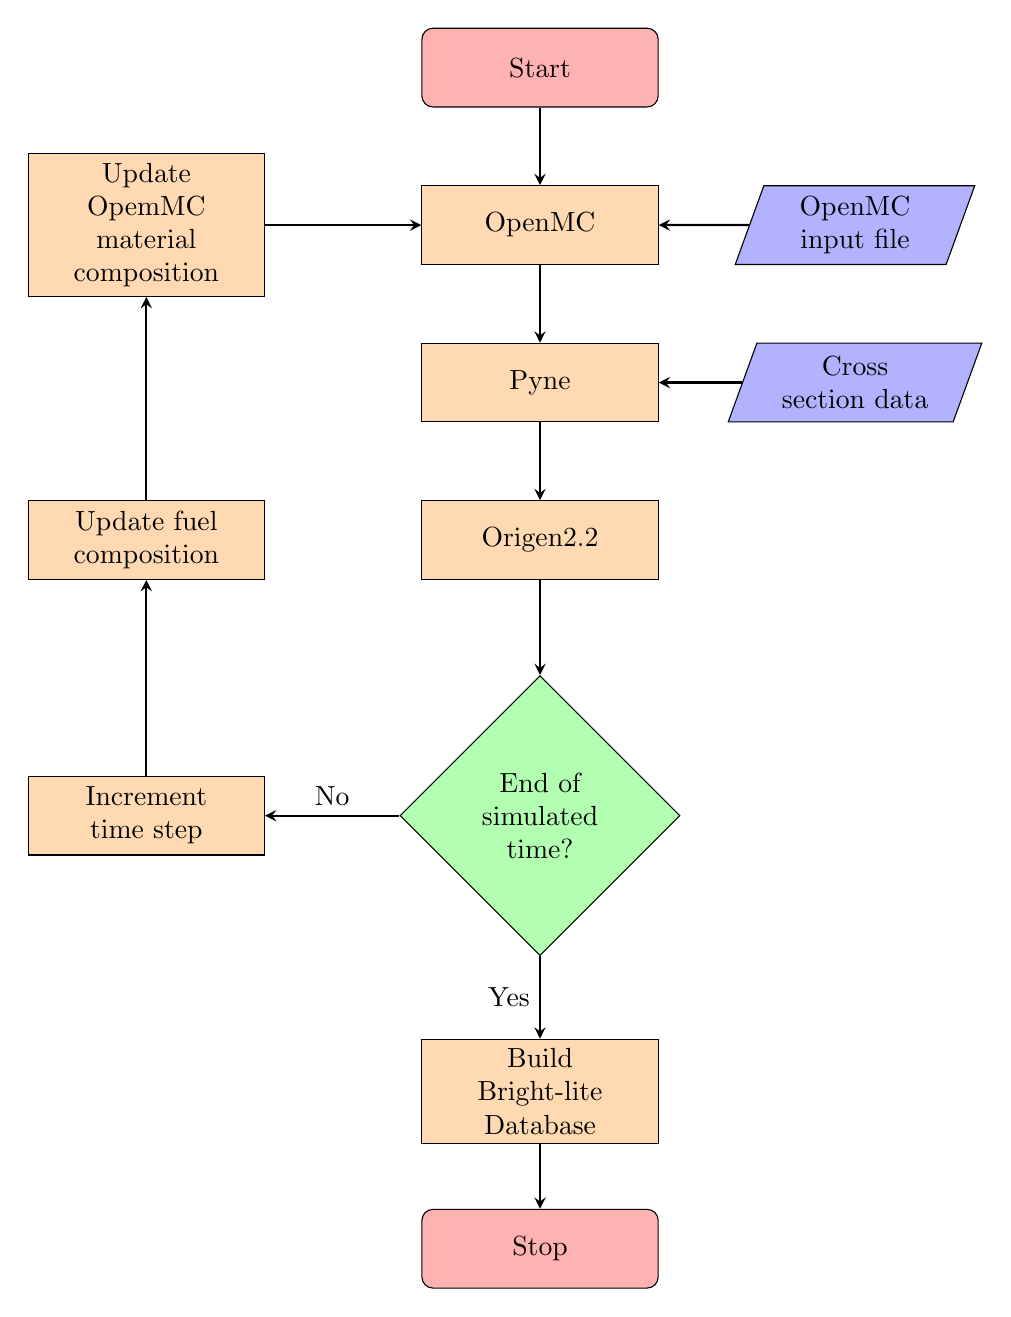
\begin{tikzpicture}[node distance=2cm]
\node (start) [startstop] {Start};
\node (openmc) [process, below of = start]{OpenMC};
\node (omcinput) [io, right of = openmc, xshift = 2cm]{OpenMC input file};
\node (omcupdate) [process, left of = openmc, xshift = -3cm]{Update OpemMC material composition};
\node (pyne) [process, below of = openmc]{Pyne};
\node (pynexs) [io, right of = pyne, xshift = 2cm]{Cross section data};
\node (origen22) [process, below of = pyne]{Origen2.2};
\node (compupdate) [process, left of = origen22, xshift = -3cm]{Update fuel composition};
\node (timecheck) [decision, below of = origen22, yshift = -1.5cm]{End of simulated time?};
\node (timeinc) [process, left of = timecheck, xshift = -3cm]{Increment time step};
\node (brightlite) [process, below of = timecheck, yshift = -1.5cm]{Build Bright-lite Database};
\node (stop) [startstop, below of = brightlite] {Stop};
\draw [arrow] (start) -- (openmc);
\draw [arrow] (omcinput) -- (openmc);
\draw [arrow] (omcupdate) -- (openmc);
\draw [arrow] (openmc) -- (pyne);
\draw [arrow] (pynexs) -- (pyne);
\draw [arrow] (pyne) -- (origen22);
\draw [arrow] (origen22) -- (timecheck);
\draw [arrow] (compupdate) -- (omcupdate);
\draw [arrow] (timeinc) -- (compupdate);
\draw [arrow] (timecheck) -- node[anchor=south]{No}(timeinc);
\draw [arrow] (timecheck) -- node[anchor=east]{Yes}(brightlite);
\draw [arrow] (brightlite) -- (stop);
\end{tikzpicture}
\caption{Flow chat of the XSgen process for building Bright-lite data tables.}
\label{fig:flow}
\end{figure}

\subsection{OpenMC}
OpenMC was used as the reference neutron transport software for modeling reactors.The software was chosen due to its availablity (it is open source), ability to quickly perform
reactor oriented calculations\citeme [journalclubarticle], and the ability to compute scattering kernels. Currently, XSgen only requires the group flux values from OpenMC, and it extracts these each timestep. Input templates for OpenMC can be specified in the XSgen run control file. 

Standard templates may also be added to XSgen itself for use in future modeling. New templates can be added to the XSgen library of reactor types by creating a new input file for OpenMC that simulates the choice reactor type. Once added to XSgen's suite of reactors the type can be accessed repeatedly. 

\subsection{PyNE}
PyNE, a Nuclear Engineering toolkit library for python, is used to perform the group collapse
from cross section databases down to the one-group or multigroup cross sections.
PyNE is capable of reading in cross section data from a wide
vareity of sources. It is able to synthesize cross section data - that may exist with
many different energy grids - down to a single energy group structure specified by the user.

The algorithm for collaspsing the cross sections, which PyNE performs in bulk, is as follows.
First, a partial energy matrix (PEM) is created. This matrix maps a higher resolution group
structures to lower resolution group structures. It does this by determining the contribution
of each of the higher resolution energy groups into the lower resolution energy groups using
a weighted sum. A PEM is only applicable for the transformation it is originally designed for. A PEM that transforms a 10 group system into a 1 group system can not be used to transform a 20 group system into a 1 group system. The calculations required to generate a PEM can be computationally expensive and therefore are only calculated if a new group structure is added to the system.  

Here, $\vec{\phi_h}$ represents the vector of group fluxes for $H$ energy groups with
a group structured defined by $E_H$ bin boundaries. Likewise, $\vec{\phi_g}$ represents
the collapsed flux with $G$ groups and $E_G$ bin boundaries. The partial energy
matrix is then defined by the relations below.

\TODO{PEM CALCULATION}

For the current use case of Bright-lite, this lower group structure is always a one group.
However, XSGen mayu generate any energy group structure desired.
Thus shifting a given group structure into a desired one using the PEM is simply a matter
of taking the dot product of the PEM by the original group structure.

\[ \vec{\phi_g} = P \cdot \vec{\phi_h} \]

Additionally, group-wise cross sections for each isotope must be calculated. This is done using the raw pointwise cross section data through the following method.

$$\sigma_{i,g}^x = \frac{\sum_{E_j=E_l}^{E_j=E_u}0.5*[\sigma(E_j)+\sigma(E_{j+1})]*[E_{j+1}-E_{j}]}{E_u-E_l}$$

Here $E_l$ and $E_u$ represent the lower and upper bounds of the energy group, $E_j$ represents the energy of a pointwise cross section in the data set, $\sigma(E_j)$ represents the cross section at energy $E_j$, and $\sigma_{i,g}^x$ represents a group wise cross section for isotope x, and cross section i.

With the one group flux ($\phi$), and group-wise cross sections, it is possible to generate the one group, flux weighted, cross sections using the following equation.

$$\sigma_{i}^x=\frac{[PEM∙(\vec{\sigma_{i,g}^x} \cdot \vec{\phi_g)}]}{\phi}$$

Here $\sigma_{i}^x$ represents the one group cross section of specific type i, for isotope x. This process is repeated for all isotopes and cross section, and those values are input into an Origin 2.2 TAPE9 file.

Pyne will also allow the user to incorperate the effects of self-shielding into XSgen. It does this build building an energy dependent function of weights of each isotope. These weights scale the one group cross section depending on the density of the isotope represented by this cross section. The more delute a isotope is within a material composition, the lower the effective cross section of the isotope. This done using the following equation.

$$\omega_{y,n}=\frac{1}{\frac{\sum_{x\neq y}N^x * \sigma_{t,g}^x}{N^y}+\sigma_{t,g}^y}$$

Here all isotopes in the fuel are included in the set of X, and Y is the isotope in question. $N_y$ represents the number density of isotope Y, and $\sigma_{t,n}^x$ represents a flux weighted total cross section of an isotope, x, in a specific energy bin, n.

Therefore similar to the mechanism described in the previous equation for calculating the one group flux weighted cross sections, these are multigroup flux weighted cross sections. Because this data is pointwise, a pointwise flux is also required. OpenMC will not output a point wise flux, so a fundamental pointwise flux is used as a supplement. The equation for this flux is as follows.

\large

\[ \phi = \begin{cases}
      \frac{2*\pi*\sqrt{E*1e6}*e^{\frac{-E*1e6}{kT}}}{(\pi*kT)^1.5} & E\leq 0.155e-6 \\
      \frac{1}{\sqrt{2E*1e6}} + 0.453e^{-1.036E}*\sinh{\sqrt{2.29E}} & E > 0.155e-6 \\
   \end{cases}
\]

Where $k$ is the Boltzman constant, $T$ is the temperature, and E is the energy. This formulation of the flux can be shown visually in Figure \ref{fig:therm}.
\begin{figure}[h]
  \center
  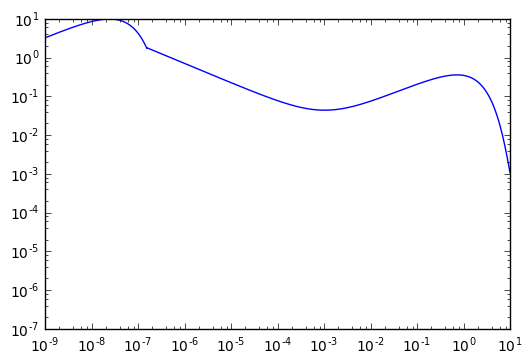
\includegraphics[scale=0.8]{thermspec.png}
  \caption{The effects of self-shielding on the cross sections for Uranium 235.}
  \label{fig:therm}
\end{figure}

The end result of all of this is a two-dimensional matrix of X (number of isotopes) by G (number of groups). The number in each entry of the matrix is the cross section weight for a specific isotope, in a specific energy group. These weights must be recalculated every time-step as the number densities of the isotopes in the fuel will charge as burnup increases.

Note, that the pointwise cross sections used in these calculation must be provided by an outside source. PyNE is capable of reading in cross sections from several different cross section libraries including; ENDF, Cinder, EAF, and OpenMC. In this case the OpenMC cross sections were used.

The effects of self shielding on U235 inside of a fuel pellet can be seen in Figure \ref{fig:index}.
\begin{figure}[h]
  \center
  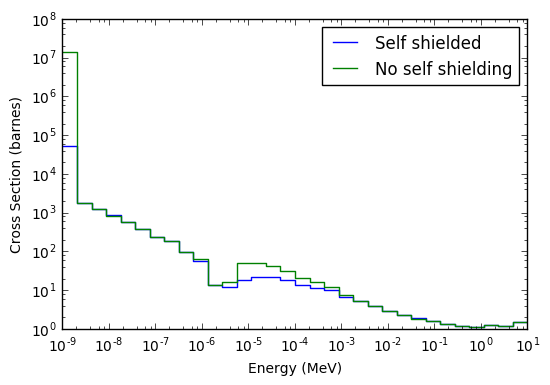
\includegraphics[scale=0.8]{index.png}
  \caption{The effects of self-shielding on the fission cross section of Uranium 235 inside a fuel pellet.}
  \label{fig:index}
\end{figure}

\subsection{Origin2.2}
Once the TAPE9 has been constructed it is used to perform two types of burnup operations. The first is performed on the fuel. This includes the full list of isotopes currently in the fuel. Once this is done the isotopic vector at the end of the fuel burn is passed back to OpenMC to start the operation all over again.

The second calculation is used to build a dataset for a specific isotope. These runs take one kilogram of a pure isotope as the input fuel. At the end of the run, the burnup, neutron production/destruction, and transmutation matrix are all recorded. The isotopes of interest are chosen ahead of time by the user of the software, these are the isotopes that the user wishes to use as the input fuel for the reactor type/design that they are investigating. 

\subsection{XSgen as a recipe generator}
Generating a recipe for a recipe reactor is done by simulating the full reactor lifetime. One technique is to use a high fidelity model to accurately model the burnup and transmutation of a reactor core from loading to discharge of a fuel assembly. 

As stated previous, XSgen also tracks a kilogram of fuel through the reactor. When this fuel goes subcritical it represents a single batch reactor core going subcritical and needing to be refueled. However, it is possible to predict the burnup of a multi-batch core from the burnup of a single batch core. The following formula shows how this might be done. 

$$ BU_n = BU_1 * (\frac{2n}{n+1}) $$

Where n is the number of batches. This technique works primarily with reactor cores that have a solid fuel that undergoes fuel shuffling during a refueling operation. Using the predicted burnup of the fuel it is possible to extract the fluence, and therefore output composition, of the fuel at that burnup. 

One thing to note about this technique is that it assumes that all batches are independent of each other. Additionally, this formula works best for reactors that have a decreasing criticality over a cycle. It would not work to provide a recipe for an accelerator driven system, or a breeder reactor. These systems aim to maintain a criticality of one as the fuel burns by breeding in new fissionable material. 

\section{Results}
\subsection{Generation results}
Figures \ref{fig:u235xs} and \ref{fig:u238xs} show cross section behavior results from running XSgen for a light water reactor using the inputs found in Table \ref{tab:xsgenstats1}. The fuel used was 3.5\% enriched uranium oxide (UOX). The number of energy groups used for this analysis was 1000. The 

\begin{table}[!htb]
\centering
\caption{Reactor details for XSgen comparisons.}
\label{tab:xsgenstats1}
\begin{tabular}{ll}
Input & Value \\
Fuel Cell Radius & 0.410 cm \\
Void Cell Radius & 0.4185 cm \\ 
clad Cell Radius & 0.475 cm \\
Unit Cell Pitch  & 1.32 cm \\
Unit Cell Height & 10.0 cm \\
Fuel Density & 10.7 [g/cc] \\
Clad Density & 5.87 [g/cc] \\
Coolant Density & 0.73 [g/cc] 
\end{tabular}
\end{table}

\begin{figure}
\caption{Cross Section Behavior of U235 in 3.5\% enriched LWR. The U235 is subjected to a constant flux of 3E14n/s/$cm^2$.}
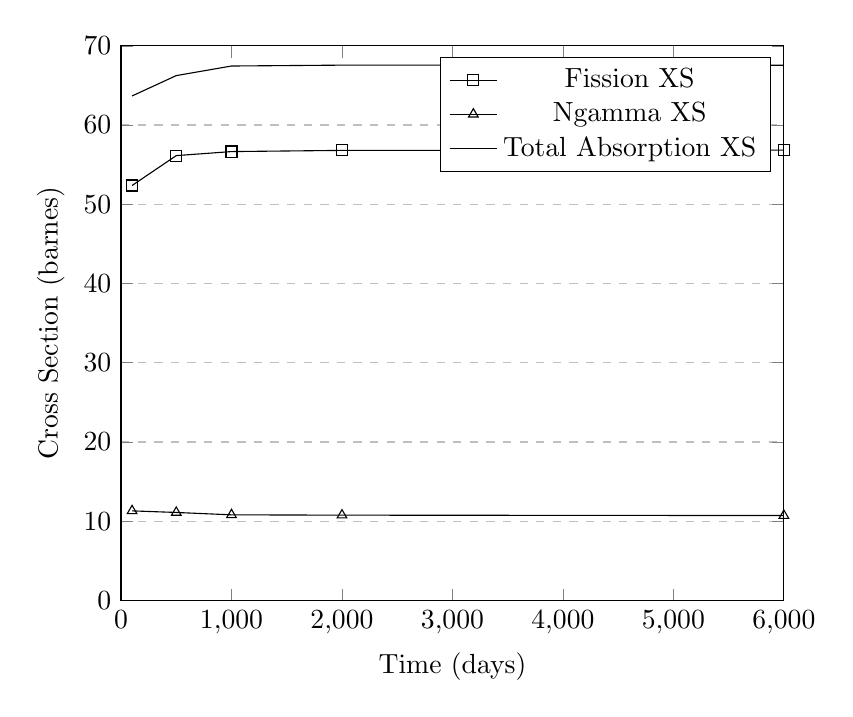
\begin{tikzpicture}
\begin{axis}[
    xlabel={Time (days)},
    ylabel={Cross Section (barnes)},
    xmin=0, xmax=6000,
    ymin=0, ymax=70,
    xtick={0,1000, 2000, 3000, 4000, 5000, 6000},
    ytick={0,10,20,30,40,50,60, 70, 80},
    ymajorgrids=true,
    grid style=dashed,
]face

\addplot[
    color=black,
    mark=square,
    ]
    coordinates {
    (100,52.37)(500,56.14)(1000,56.65)(2000,56.80)(6000,56.84)
    };
    \addlegendentry{Fission XS}
\addplot[
    color=black,
    mark=triangle,
    ]
    coordinates {
    (100,11.3)(500,11.1)(1000,10.8)(2000,10.76)(6000,10.71)
    };
    \addlegendentry{Ngamma XS}
\addplot[
    color=black,
    mark=circle,
    ]
    coordinates {
    (100,63.67)(500,66.24)(1000,67.45)(2000,67.56)(6000,67.55)
    };
    \addlegendentry{Total Absorption XS}
\end{axis}
\label{fig:u235xs}
\end{tikzpicture}
\end{figure}

\begin{figure}
\caption{Cross Section Behavior of U238 in 3.5\% enriched LWR. The U238 is subjected to a constant flux of 3E14n/s/$cm^2$.}
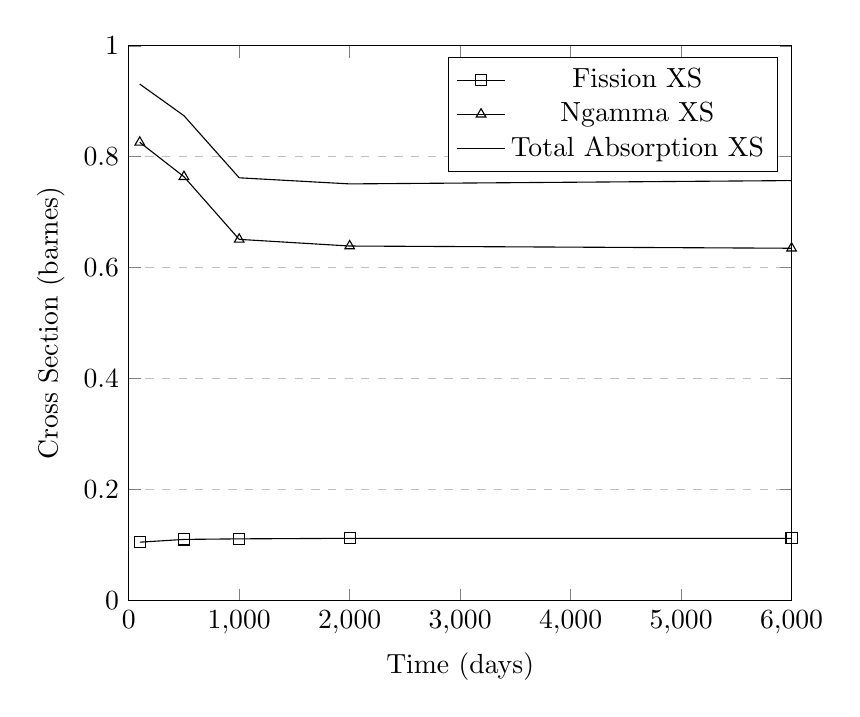
\begin{tikzpicture}
\begin{axis}[
    xlabel={Time (days)},
    ylabel={Cross Section (barnes)},
    xmin=0, xmax=6000,
    ymin=0, ymax=1,
    xtick={0,1000, 2000, 3000, 4000, 5000, 6000},
    ytick={0,0.20,0.4,0.6,0.8,1.0},
    ymajorgrids=true,
    grid style=dashed,
]
\addplot[
    color=black,
    mark=square,
    ]
    coordinates {
    (100,0.105)(500,0.11)(1000,0.111)(2000,0.112)(6000,0.112)
    };
    \addlegendentry{Fission XS}
\addplot[
    color=black,
    mark=triangle,
    ]
    coordinates {
    (100,0.826)(500,0.764)(1000,0.651)(2000,0.639)(6000,0.635)
    };
    \addlegendentry{Ngamma XS}
\addplot[
    color=black,
    mark=circle,
    ]
    coordinates {
    (100,0.931)(500,0.874)(1000,0.762)(2000,0.751)(6000,0.757)
    };
    \addlegendentry{Total Absorption XS}
\end{axis}
\label{fig:u238xs}
\end{tikzpicture}
\end{figure}

The two figures (\ref{fig:U235xs}, \ref{fig:U238xs})the the cross section changes slowly over the course of operating the reactor. This is to be expected as the flux and number density of these two isotopes changes. U235 and U238 both undergo a net burn effect, which is why you see the behavior of the cross sections for these two isotopes change in similar ways over the course of the XSgen simulation. This behavior is inline with the expected behavior of cross sections within a light water reactor. 

Additionally the following figure shows the equalibrium flux of the reactors as determined by OpenMC. 
Figure \ref{fig:32g} shows the fluxes of the same XSgen run using two different energy group structures; 32, and 1000.  

\begin{figure}[h]
  \center
  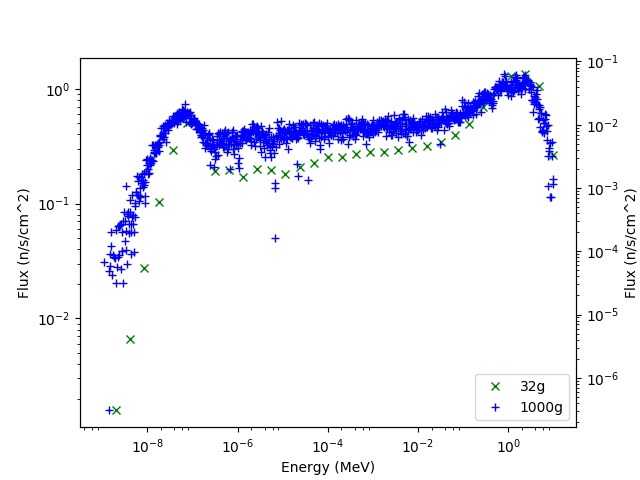
\includegraphics[scale=0.7]{fluxes.png}
  \caption{Fluxes generated by OpenMC for a light water reactor using 32 and 1000 group energy structures.}
  \label{fig:32g}
\end{figure}

Figure \ref{fig:32g} shows the expected behavior between the two group structures. The larger group structure manages to catch the effects of some of stronger resonance groups as well as providing better detail to the lower group structures. 

\subsection{LWR Benchmarking Cases}
XSgen by itself can not directly be tested against operating reactor systems. It was originally designed to produce datasets a medium fidelity reactor model known as Bright-lite. Therefore, to benchmark XSgen it will be used in conjunction with Bright-lite to produce burnups and isotopes for several known reactor systems.  As Bright-lite has already been benchmarked several times using other datasets\cite{brightlite} it is assumed that the operations within Bright-lite are accurate and any deviations within the results come from XSgen.

The most well studied reactors in the world are light water reactors and as such these will be used as benchmarking tools for XSgen. Primarily the cases represent a range of different enrichments in several light water reactors, comparing the results from XSgen/Bright-lite to recipes from VISION\cite{vision}. Additionally, the values will be tested against two cases modelling reactor startup behavior. 

The XSgen/Bright-light will be benchmarked against VISION at 3.0, 3.5, and 4.0 percent enrichment. Three batch cores will be assumed for all the enrichment test cases.
The two cases being used to test XSgen in startup behavior will be a 3.1$\%$ enriched light water reactor using four batches and a 3.6$\%$ enriched light water reactor using four batches. The cases will be compared using burnups, isotopic composition of fresh and used fuel.

\begin{table}[!htb]
\centering
\small
\caption{The output isotopics at equalibrium for the VISION fuel cycle simulator}
\label{tab:a}
\vspace{0.5em}
\begin{tabular}{cccc}
 & \multicolumn{1}{c}{3.0\%} & \multicolumn{1}{c}{3.5\%} & \multicolumn{1}{c}{4.0\%} \\
Isotope & Mass Fraction & Mass Fraction & Mass Fraction \\
\hline
U235  & 6.75E-3 & 6.80E-3 & 6.95E-3 \\
Pu238 & 1.23E-4 & 1.85E-4 & 2.52E-4 \\
Pu239 & 5.15E-3 & 5.41E-3 & 5.64E-3 \\
Pu240 & 2.38E-3 & 2.60E-3 & 2.78E-3 \\
Pu241 & 1.30E-3 & 1.48E-3 & 1.62E-3 \\
Pu242 & 5.43E-4 & 6.92E-4 & 8.17E-4 \\
Am241 & 3.56E-5 & 4.59E-5 & 5.55E-5 \\
Am243 & 9.38E-5 & 1.37E-4 & 1.76E-4 \\
Cm242 & 1.38E-5 & 1.88E-5 & 2.33E-5 \\
Cm244 & 2.79E-5 & 4.38E-5 & 7.06E-5 \\
\hline
\end{tabular}
\end{table}

\begin{table}[!htb]
\centering
\small
\caption{A comparison of the output isotopics at equalibrium in the VISION fuel cycle simulator and the XSgen-Bright-lite system. Comparison is done as a percent difference.}
\label{tab:xsgenresults}
\vspace{0.5em}
\begin{tabular}{c cc  cc  cc }
 & \multicolumn{2}{c}{3.0\%} & \multicolumn{2}{c}{3.5\%} & \multicolumn{2}{c}{4.0\%} \\
Isotope & Bright-lite & Difference & Bright-lite & Difference & Bright-lite & Difference  \\
\hline
U235 & 6.70E-3 & -0.78 & 6.71E-3 & -1.30 & 6.91E-3 & -0.562 \\
Pu238 & 1.27E-4 & 3.01 & 1.86E-4 & -0.41 & 2.55E-4 & 1.35 \\
Pu239 & 5.25E-3 & 1.95 & 5.45E-3 & 0.66 & 5.67E-3 & 0.57 \\
Pu240 & 2.40E-3 & 0.97 & 2.61E-3 & 0.25 & 2.79E-3 & 0.4 \\
Pu241 & 1.35E-3 & 3.69 & 1.52E-3 & 2.74 & 1.62E-3 & -0.02 \\
Pu242 & 5.48E-4 & 0.88 & 6.93E-4 & 0.10 & 8.19E-4 & -0.28 \\
Am241 & 3.86E-5 & 8.81 & 5.17E-5 & 12.60 & 6.04E-5 & 8.79 \\
Am243 & 9.01E-5 & -3.94 & 1.26E-4 & -7.47 & 1.74E-4 & -1.40 \\
Cm242 & 1.34E-5 & -3.19 & 1.79E-5 & -4.91 & 2.31E-5 & -0.83 \\
Cm244 & 2.57E-5 & -7.94 & 4.54E-5 & -6.06 & 7.00E-5 & -0.90 \\
\hline
\end{tabular}
\end{table}

Table \ref{tab:a} shows the output composition for three different fuel enrichments discussed. These outputs are used as a basis for comparison for Table \ref{tab:xsgenresults}.

Table \ref{tab:xsgenresults} shows a very strong agreement between VISION and Bright-light results using datasets created from light water reactors designed to these particular enrichments. Bright-light has been benchmarked against VISION previously using other datasets. This shows that given XSgen generated datasets allows for Bright-lite to match VISION to a 5\% tolence for a majority of isotopes. Those that exhibit the greatest deviations are high order transuranics.

Am241 shows the largest deviations from the VISION data. There is more Am241 in every case than expected by the VISION results, and less of the species that are arise due to the presence of Am241; Am243, Cm242, Cm244. These results can be explained by a neutron absorption cross section error in Am241. If the neutron absorption cross section for Am241 is too low it can never transmute into Am242 and Am243, which in turn leads to an absence of curium isotopes.

Additionally the Bright-lite model generated by XSgen was tested against a set of Nuclear Enegy Agency (NEA) results\cite{nea}. These results show the start up behavior of the same reaction using two different fuel enrichments. 

\subsection{LWR Startup Behavior Benchmarking}
\begin{table}[!htb]
\centering
\caption{NEA core discharge data for a 3.1\% enriched light water reactor with startup behavior.}
\label{tab:b}
\begin{tabular}{lrrrr}
Batch & Burnup (MWd/kg) & U235 (\%) & Fissile Pu (\%) & Total Pu(\%) \\
1 & 12.04 & 0.64 & 0.464 & 0.633 \\
2 & 23.86 & 0.76 & 0.6 & 0.818 \\
3 & 31.75 & 0.8 & 0.677 & 0.921 \\
4 & 32.00 & 0.85 & 0.697 & 0.943 \\
Equil. & 33.00 & 0.85 & 0.688 & 0.943
\end{tabular}
\end{table}

\begin{table}[!htb]
\centering
\caption{The startup values and percent difference from the NEA data for the XSgen/Bright-lite reactor system.}
\label{tab:c}
\begin{tabular}{lrrrrrrrr}
 & \multicolumn{2}{p{1cm}}{Burnup (MWd/kgIHM)} & \multicolumn{2}{c}{U235 (\%)} & \multicolumn{2}{c}{Fissile Pu (\%)} & \multicolumn{2}{c}{Total Pu (\%)} \\
Batch & Value & \%Diff & Value & \%Diff & Value & \%Diff & Value & \%Diff \\
1 & 13.570 & 12.754 & 0.656 & 2.50 & 0.550 & 18.737 & 0.680 & 7.541 \\
2 & 22.040 & -7.628 & 0.723 & -4.868 & 0.641 & 6.919 & 0.835 & 2.189 \\
3 & 32.510 & 2.394 & 0.789 & -1.375 & 0.710 & 4.883 & 0.970 & 5.231 \\
4 & 31.230 & -2.406 & 0.851 & 0.117 & 0.680 & -2.254 & 0.906 & -5.031 \\
5 & 33.010 & 0.030 & 0.843 & -0.824 & 0.703 & 2.198 & 0.946 & 0.285 \\
Equal. & 33.020 & 0.060 & 0.855 & 0.588 & 0.700 & 1.833 & 0.951 & 0.820
\end{tabular}
\end{table}

Table \ref{tab:b} shows how XSgen/Bright-lite compares to the NEA results. The equilibrium results here show good agreement with this case. As Bright-lite is often used to derive output isotopics from used fuels to be passed onto recycle scenarios, accurately predicting the equilibrium output isotopics is important.

The results of the start up isotopics can be seen in Table \ref{tab:c}. There are some discrepencies in these results. First, the amount of plutonium generated within the first batch is significantly higher within Bright-lite compared to the NEA data. This trend only continues for the first two cycles. Due to the way Bright-lite operates, this is caused by the lower enriched batches within the startup core that do not have neutron poisons from fission products or other actinides. This means that there is a higher effective flux striking a high amount of U238 causing more generation of Pu239. The NEA benchmark has these low enrichment startup batches spread more evenly, Bright-lite simulates them as being the innermost section of the core. 

\begin{table}[!htb]
\centering
\caption{NEA data for a 3.6\% enriched light water reactor start up behavior.}
\label{tab:d}
\begin{tabular}{lllll}
Batch & Burnup (MWd/kg) & U235 (\%) & Fissile Pu (\%) & Total Pu(\%) \\
1 & 13.9 & 0.840 & 0.474 & 0.629 \\
2 & 22.67 & 0.721 & 0.642 & 0.892 \\
3 & 32.36 & 0.647 & 0.716 & 1.039 \\
4 & 41.00 & 0.640 & 0.785 & 1.177 \\
5 & 39.00 & 0.940 & 0.808 & 1.166 \\
6 & 40.60 & 0.88 & 0.817 & 1.194 \\
Equil. & 42.50 & 0.81 & 0..827 & 1.223
\end{tabular}
\end{table}

\begin{table}[!htb]
\centering
\caption{XSgen / Bright-lite data for the 3.6\% enriched light water reactor start up behavior.}
\label{tab:e}
\begin{tabular}{lllllllll}
 & \multicolumn{2}{l}{Burnup (MWd/kgIHM)} & \multicolumn{2}{l}{U235 (\%)} & \multicolumn{2}{l}{Fissile Pu (\%)} & \multicolumn{2}{l}{Total Pu (\%)} \\
Batch & Value & \%Diff & Value & \%Diff & Value & \%Diff & Value & \%Diff \\
1 & 13.37 & -3.84 & 0.930 & 10.77 & 0.62 & 30.43 & 0.78 & 23.53 \\
2 & 22.69 & 0.07 & 0.82 & 13.02 & 0.72 & 12.81 & 0.96 & 7.49 \\
3 & 32.38 & 0.03 & 0.72 & 11.08 & 0.78 & 8.46 & 1.07 & 2.69 \\
4 & 42.57 & 3.83 & 0.61 & -5.33 & 0.804 & 2.42 & 1.14 & -2.94 \\
5 & 41.00 & 5.13 & 0.85 & 9.526 & 0.79 & -2.81 & 1.10 & -5.91 \\
6 & 43.83 & 3.04 & 0.82 & 6.53 & 0.79 & -3.58 & 1.11 & -7.45 \\
Equal. & 42.32 & -0.43 & 0.81 & -0.44 & 0.79 & -4.54 & 1.11 & -9.42
\end{tabular}
\end{table}

Table \ref{tab:d} and Table \ref{tab:e} are repeats of Table \ref{tab:b} and Table \ref{tab:c} for the 3.6$\%$ enriched light water reactor. Again, you see a similar trend in these two with the exception that the equilibrium results for the total amount of plutonium within the reactor is 9.2$\%$ lower in the Bright-lite model. The amount of fissile plutonium is also lower, but within acceptable bounds. The lower amount of fissile plutonium leads to less transmutations into the high order actinides.

\subsection{MOX Case Benchmarking}
Simply replicating the behavior of a light water reactor would not show off the full capabilities of the XSgen software. To demonstrate the capability of the system to extend to more advanced reactor types, XSgen will be used to generate a MOX fuel library for Bright-lite. It will then be used to simulate a single pass MOX reactor. In order to compare this on an apples to apples basis, the input fuel into the Bright-lite reactor will be exactly the same as that for a similar VISION reactor. This test will be able to demonstrate the flexibility of the combined XSgen/Bright-lite system that allows it to model advanced reactor types.

\begin{table}[!htb]
\centering
\caption{Comparison of VISION and Bright-lite result from a single pass MOX reactor.}
\label{tab:g}
\begin{tabular}{lllll}
Isotope & Input Composition & Vision & Bright-lite & Difference(\%) \\
U234 & 2.20E-4 & 2.11E-4 & 2.00E-4 & -5.0\\
U235 & 7.08E-3 & 4.05E-3 & 4.00E-3 & -1.2\\
U236 & 5.28E-3 & 4.97E-3 & 5.60E-3 & 12.6\\
U238 & 8.80E-1 & 8.51E-1 & 8.62E-1 & 1.3\\
Pu238 & 2.85E-3 & 3.22E-3 & 3.01E-3 & -6.5\\
Pu239 & 5.66E-2 & 3.31E-2 & 3.15E-2 & -4.6\\
Pu240 & 2.70E-2 & 2.42E-2 & 2.54E-2 & 5.0\\
Pu241 & 1.17E-2 & 1.31E-2 & 1.27E-2 & -3.3\\
Pu242 & 8.00E-3 & 8.90E-3 & 8.68E-3 & -2.6\\
Am241 & 1.18E-3 & 1.72E-3 & 1.60E-3 & -7.2\\
Am243 & - & 1.96E-3 & 1.83E-3 & -6.6\\
Cm242 & - & 2.62E-4 & 2.46E-4 & -6.4\\
CM244 & - & 1.03E-3 & 9.84E-4 & -4.4
\end{tabular}
\end{table}

The data in Table \ref{tab:g} shows that the results of Bright-lite given the new XSgen MOX reactor cross section fairs quite well compared to VISION. There are some outliers in the behaviors, specifically the higher order species and U236. The issues with the higher order actinides, Am241 and higher, most likely stem from the high amount of Pu240. This suggest that Pu240 is not transmuting into Pu241 at a high enough rate, which therefore lowers the equalibrium concentration of Pu241 and all isotopes that derive from it.

One of the possible primary causes of this is uncertainity in the exact dimensions and behavior of the VISION MOX reactor. In order to get the most accurate results XSgen needs to know the specification of the MOX reactor. Instead for this work a generic 17x17 light water reactor core was chosen to use as a base for the XSgen run. If the input and output compositions generated for VISION were made from a reactor core of a different design it would result in slightly different cross sections and therefore different behavior.

\subsection{Recipe Reactor Generation}
As discussed above, XSgen can be used to create recipe reactors as well. The following results show a comparison between VISION and XSgen recipe reactors. These reactors use a 3.2\% U235 enriched fuel. The XSgen model assumes the information found in Table \ref{tab:xsgenstats} about the reactor. 
 
\begin{table}[!htb]
\centering
\caption{Comparison of VISION and XSgen for the generation of a 33 MWd/kgIHM Burnup.}
\label{tab:xsgenstats}
\begin{tabular}{ll}
Input & Value \\
Fuel Cell Radius & 0.410 cm \\
Void Cell Radius & 0.4185 cm \\ 
clad Cell Radius & 0.475 cm \\
Unit Cell Pitch  & 1.32 cm \\
Unit Cell Height & 10.0 cm \\
Fuel Density & 10.7 [g/cc] \\
Clad Density & 5.87 [g/cc] \\
Coolant Density & 0.73 [g/cc] 
\end{tabular}
\end{table}

Table \ref{tab:recipe} shows the difference between the VISION 3.2\% light water reactor and the XSgen version of that reactor. 

\begin{table}[!htb]
\centering
\caption{Comparison of VISION and XSgen for the generation of a 33 MWd/kgIHM Burnup.}
\label{tab:recipe}
\begin{tabular}{llllll}
Isotope & Vision & XSgen & Difference(\%) \\
U235 & 8.06E-03 & 7.84E-03 & -2.85 \\
U238 & 9.44E-01 & 9.67E-01 & 2.36 \\
Pu238 & 1.09E-04 & 1.01E-04 & -7.80 \\
Pu239 & 5.13E-03 & 4.83E-03 & -6.15 \\
Pu240 & 2.25E-03 & 2.41E-03 & 6.52 \\
Pu241 & 1.22E-03 & 1.17E-03 & -4.53 \\ 
Pu242 & 4.73E-04 & 4.49E-04 & -5.26 \\
Am241 & 2.98E-05 & 2.76E-05 & -7.97 \\
Am243 & 7.90E-05 & 7.23E-05 & -9.31 \\
Cm242 & 1.17E-05 & 1.07E-05 & -9.48 \\
Cm244 & 2.22E-05 & 2.11E-05 & -5.11 \\
\end{tabular}
\end{table}

The results in Table \ref{tab:recipe} show that XSgen is with 10\% error on all output isotopics for this reactor design. There are two possible causes of this issue. The first is the method used for extrapolating the data for a multi-batch core from a single batch core. Additionally, the design of the VISION reactor is unknown. This means that the reactor modeled with XSgen may not be a perfect one to one match with the reactor model used for VISION.  

\section{Conclusion}
The work of nuclear reactor models is to provide researchers with insight into the behavior of reactors and by extension nuclear fuel cycles. Comparisons between these models is important to understanding how the choice of model might impact the accuracy of the results. Through this work XSgen has demonstrated that it is capable of providing a method of generating one-group cross sections and a number of reactor parameters using benchmarked software. This provides a path forward for generating datasets for medium and low fidelity models such that they may all be compared on an equal footing. This will allow researchers to understand how these models affect the results of fuel cycle analysis. 

Additionally XSgen provides a method for automating the generation of reactor types for medium fidelity models. The work here linking XSgen to the Bright-lite reactor model shows that XSgen can be used to expand the set of reactor types and reactor designs (i.e. varied burnups, enrichment, or core structure) that Bright-lite has access to. Through this coupling Bright-lite can be used to quickly example fuel cycles with new or interesting reactor technologies. Future work should aim to expand this coupling to include other medium fidelity models as well.


\bibliography{xsgen} 
\bibliographystyle{ieeetr}

\end{document}

